\section{本研究で用いるプレイヤ}
\subsection{Nタプルネットワーク評価関数}
\label{sec:Ntuple}

2048における最も成功したプレイヤの多くは、Nタプルネットワークに基づく評価関数を強化学習によってチューニングするアプローチを採用している~\cite{SzJa14}。
Gueiらの最新のプレイヤ~\cite{GuCW22}も、Matsuzaki~\cite{Mats16}が提案したタプルの組合せをベースに、Expectimax探索やMultistaging\cite{YWHC16}、Optimistic Initialization、Tile Downgrading\cite{GuCW22}などの改良を加えることで高い性能を達成している。

本研究では、こうした知見を踏まえ、ミニ2048において1タプルから9タプルまでのNタプルネットワークを構築可能な全てのタプル列挙を行い、
\begin{itemize}
  \item 我々が妥当と判断した形状のみを選んだタプル集合
  \item 各サイズごとの連続タイルすべてを使用したタプル集合
\end{itemize}
    という2通りの設計方針でネットワークを構築した。

この結果、最大で18種類のNタプルネットワークが得られたが、1タプル、2タプル、9タプルにおいては両方の設計が一致したため、プレイヤの種類としては15通りとなった。
これらのプレイヤを用いて、Nタプルネットワークの大きさ(タプル数)と学習性能の関係を実験的に評価した。

表\ref{tuples}に、本研究で使用したタプルの構造を示す。
また、ミニ2048の盤面の持つ対称性(回転・反転)**を活用し、1つのタプルに対して対称な8通りの位置からのサンプリングを行うことで、学習に必要なタプル数の削減を図っている。

\begin{table}[t]
  \caption{タプルサイズと形状の一覧}
  \label{tuples}
  \centering\begin{tabular}{ll}
   \hline
   \hline
   タプル名 & \hspace{20pt}タプルの形状 \\
   \hline
   \raisebox{10pt}{NT1F}\raisebox{28pt}{~}
          & 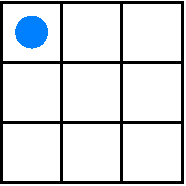
\includegraphics[height=22pt]{pdf/tuples/1tuple_6_page1.pdf}~
            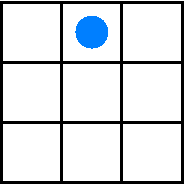
\includegraphics[height=22pt]{pdf/tuples/1tuple_6_page2.pdf}~
            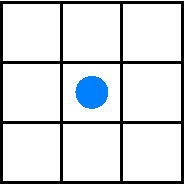
\includegraphics[height=22pt]{pdf/tuples/1tuple_6_page3.pdf}\\
   \hline
   \raisebox{10pt}{NT2F}\raisebox{28pt}{~}
          & 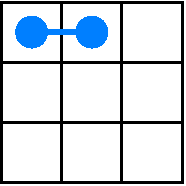
\includegraphics[height=22pt]{pdf/tuples/2tuple_12_page1.pdf}~
            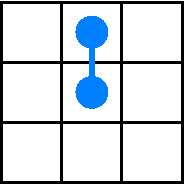
\includegraphics[height=22pt]{pdf/tuples/2tuple_12_page2.pdf}\\
   \hline
   \raisebox{10pt}{NT3M}\raisebox{28pt}{~}
          & 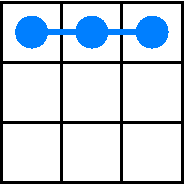
\includegraphics[height=22pt]{pdf/tuples/3tuple_144_page1.pdf}~
            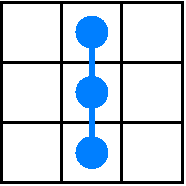
\includegraphics[height=22pt]{pdf/tuples/3tuple_144_page3.pdf}~
            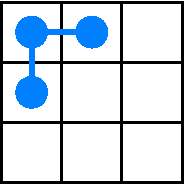
\includegraphics[height=22pt]{pdf/tuples/3tuple_144_page2.pdf}\\
   \hline
   \raisebox{10pt}{NT3F}\raisebox{28pt}{~}
          & 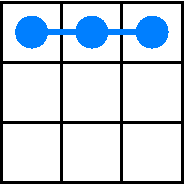
\includegraphics[height=22pt]{pdf/tuples/3tuple_2673_page1.pdf}~
            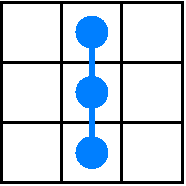
\includegraphics[height=22pt]{pdf/tuples/3tuple_2673_page5.pdf}~
            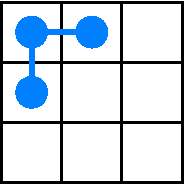
\includegraphics[height=22pt]{pdf/tuples/3tuple_2673_page2.pdf}~
            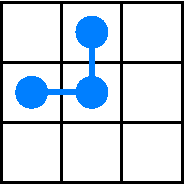
\includegraphics[height=22pt]{pdf/tuples/3tuple_2673_page4.pdf}~
            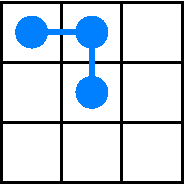
\includegraphics[height=22pt]{pdf/tuples/3tuple_2673_page3.pdf}\\
   \hline
   \raisebox{10pt}{NT4M}\raisebox{28pt}{~}
          & 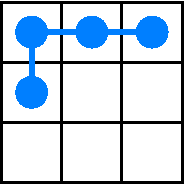
\includegraphics[height=22pt]{pdf/tuples/4tuple_301_page1.pdf}~
            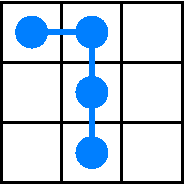
\includegraphics[height=22pt]{pdf/tuples/4tuple_301_page3.pdf}~
            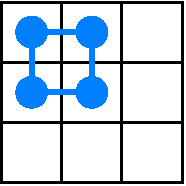
\includegraphics[height=22pt]{pdf/tuples/4tuple_301_page2.pdf}\\
   \hline
   \raisebox{10pt}{NT4F}\raisebox{28pt}{~}
          & 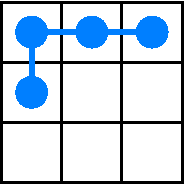
\includegraphics[height=22pt]{pdf/tuples/4tuple_44755_page1.pdf}~
            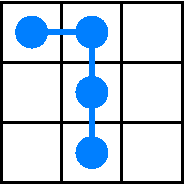
\includegraphics[height=22pt]{pdf/tuples/4tuple_44755_page5.pdf}~
            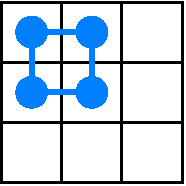
\includegraphics[height=22pt]{pdf/tuples/4tuple_44755_page3.pdf}\\
          & 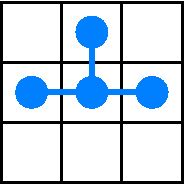
\includegraphics[height=22pt]{pdf/tuples/4tuple_44755_page6.pdf}~
            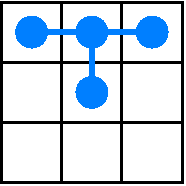
\includegraphics[height=22pt]{pdf/tuples/4tuple_44755_page2.pdf}~
            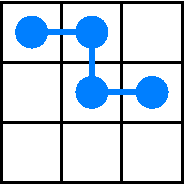
\includegraphics[height=22pt]{pdf/tuples/4tuple_44755_page4.pdf}\\
   \hline
   \raisebox{10pt}{NT5M}\raisebox{28pt}{~}
          & 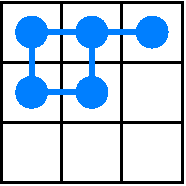
\includegraphics[height=22pt]{pdf/tuples/5tuple_298_page1.pdf}~
            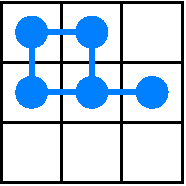
\includegraphics[height=22pt]{pdf/tuples/5tuple_298_page2.pdf}~
            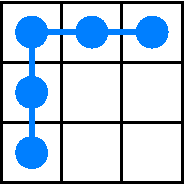
\includegraphics[height=22pt]{pdf/tuples/5tuple_298_page3.pdf}\\
   \hline
   \raisebox{10pt}{NT5F}\raisebox{28pt}{~}
          & 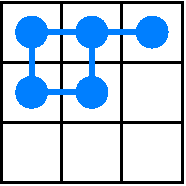
\includegraphics[height=22pt]{pdf/tuples/5tuple_896673_page1.pdf}~
            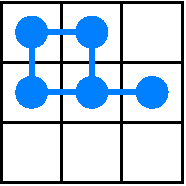
\includegraphics[height=22pt]{pdf/tuples/5tuple_896673_page3.pdf}~
            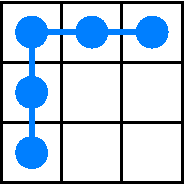
\includegraphics[height=22pt]{pdf/tuples/5tuple_896673_page4.pdf}~
            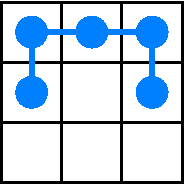
\includegraphics[height=22pt]{pdf/tuples/5tuple_896673_page2.pdf}~
            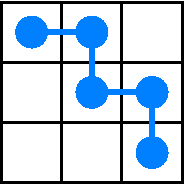
\includegraphics[height=22pt]{pdf/tuples/5tuple_896673_page5.pdf}\\
          & 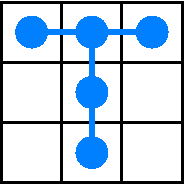
\includegraphics[height=22pt]{pdf/tuples/5tuple_896673_page6.pdf}~
            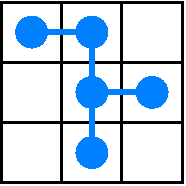
\includegraphics[height=22pt]{pdf/tuples/5tuple_896673_page7.pdf}~
            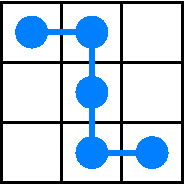
\includegraphics[height=22pt]{pdf/tuples/5tuple_896673_page8.pdf}~
            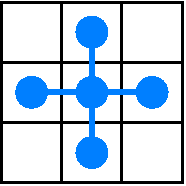
\includegraphics[height=22pt]{pdf/tuples/5tuple_896673_page9.pdf}\\
   \hline
   \raisebox{10pt}{NT6M}\raisebox{28pt}{~}
          & 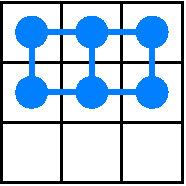
\includegraphics[height=22pt]{pdf/tuples/6tuple_16_page1.pdf}~
            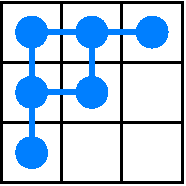
\includegraphics[height=22pt]{pdf/tuples/6tuple_16_page2.pdf}\\
   \hline
   \raisebox{10pt}{NT6F}\raisebox{28pt}{~}
          & 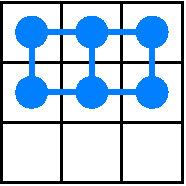
\includegraphics[height=22pt]{pdf/tuples/6tuple_26835_page1.pdf}~
            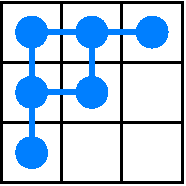
\includegraphics[height=22pt]{pdf/tuples/6tuple_26835_page2.pdf}~
            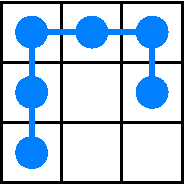
\includegraphics[height=22pt]{pdf/tuples/6tuple_26835_page3.pdf}~
            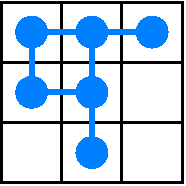
\includegraphics[height=22pt]{pdf/tuples/6tuple_26835_page4.pdf}\\
          & 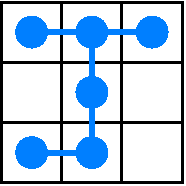
\includegraphics[height=22pt]{pdf/tuples/6tuple_26835_page5.pdf}~
            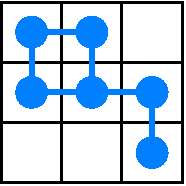
\includegraphics[height=22pt]{pdf/tuples/6tuple_26835_page6.pdf}~
            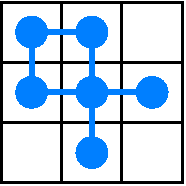
\includegraphics[height=22pt]{pdf/tuples/6tuple_26835_page7.pdf}~
            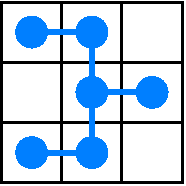
\includegraphics[height=22pt]{pdf/tuples/6tuple_26835_page8.pdf}\\
   \hline
   \raisebox{10pt}{NT7M}\raisebox{28pt}{~}
          & 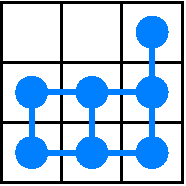
\includegraphics[height=22pt]{pdf/tuples/7tuple_0_page1.pdf}\\
   \hline
   \raisebox{10pt}{NT7F}\raisebox{28pt}{~}
          & 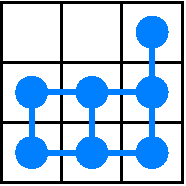
\includegraphics[height=22pt]{pdf/tuples/7tuple_248_page1.pdf}~
            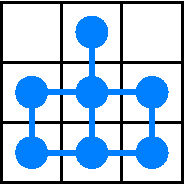
\includegraphics[height=22pt]{pdf/tuples/7tuple_248_page2.pdf}~
            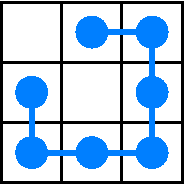
\includegraphics[height=22pt]{pdf/tuples/7tuple_248_page3.pdf}~
            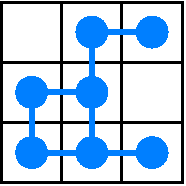
\includegraphics[height=22pt]{pdf/tuples/7tuple_248_page4.pdf}\\
          & 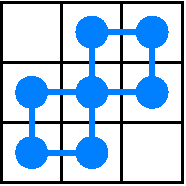
\includegraphics[height=22pt]{pdf/tuples/7tuple_248_page5.pdf}~
            \includegraphics[height=22pt]{pdf/tuples/7tuple_248_page6.pdf}~
            \includegraphics[height=22pt]{pdf/tuples/7tuple_248_page7.pdf}\\
   \hline
   \raisebox{10pt}{NT8M}\raisebox{28pt}{~}
          & \includegraphics[height=22pt]{pdf/tuples/8tuple_0_page1.pdf}\\
   \hline
   \raisebox{10pt}{NT8F}\raisebox{28pt}{~}
          & \includegraphics[height=22pt]{pdf/tuples/8tuple_6_page1.pdf}~
            \includegraphics[height=22pt]{pdf/tuples/8tuple_6_page2.pdf}~
            \includegraphics[height=22pt]{pdf/tuples/8tuple_6_page3.pdf}\\
   \hline
   \raisebox{10pt}{NT9F}\raisebox{28pt}{~}
          & \includegraphics[height=22pt]{pdf/tuples/9tuple_0_page1.pdf}\\
   \hline
  \end{tabular}
\end{table}

Nタプルネットワークの重みは,afterstate 間の評価値の差に基づくTD学習法の改良手法によって調整した.
本研究で用いるNタプルネットワークの学習では,以下の技術を用いた.
\begin{description}
  % \item [対称性サンプリング] 各タプルについて,鏡面,回転対称用いてを1つの盤面から,8つの対称位置からサンプリングする. これにより,少ないタプル数で盤面全体から特徴を抽出することができる.
  \item [Multistaging] ゲームの進行に応じて重みを参照するテーブルを切り替える.本研究では,2ステージとし,512 のタイルができる前後でステージを分けた.
  \item [Temporal coherence 学習(TC学習)] TC学習は学習率自動調整機能を備えたTD学習で,Ja\'{s}kowski~\cite{Jask17}が始めて2048に導入した.
  \item [Optimistic initialization] 学習段階での探索を広く行うために,重みを(ゼロではなく)大きな値で初期化する.本研究で用いたNタプルの学習では,すべての afterstate の初期値が 1200 になるように重みを初期化してある.
\end{description}

それぞれのNタプルニューラルネットワークに対して,$5\times 10^8$ 局面分のデータで学習を行った.いずれのニューラルネットワークも,十分に学習が収束していることを確認してある~\cite{TeKM23}.
% \newpage
\section{Expectimax探索}
\label{sec:expectimax}
Expectimax探索は,確率的一人ゲームにおける標準的な探索手法である.
ミニ2048のゲームの進行は,state におけるプレイヤの選択と,afterstate における新規タイルの出現が交互に起こる.
したがって,ミニ2048のゲーム木は,根が現在の state に対応し,根から葉への各パス上に,afterstate に対応するノード(chance ノード)と state に対応するノード(max ノード)が交互に現れる.本研究では,ミニ2048のゲーム木の高さ(探索の深さ)を,各パス上の afterstate に対応するノードの数と定める.例えば,高さ2 のミニ2048のゲーム木は,根,afterstate に対応するノードの層,state に対応するノードの層,afterstate に対応するノードの層,の合計4層からなる(図~\ref{result.Expectimax}).

Expectimax探索では,ゲーム木の各ノードに対して次のように再帰的に計算を行う.
\begin{itemize}
 \item maxノードでは,子要素の値のうちの最大値を計算する.
 \item chanceノードでは,子要素の値を,その出現確率を用いた重み付き平均を計算する.
\end{itemize}
Expectimax探索プレイヤは,Expectimax探索によって得られた子ノードのうち,評価値の最も大きなものを選択する.

図\ref{result.Expectimax}に深さ2のExpectimax探索の例を示す.

\begin{figure}[t]
  \centering
  \includegraphics[width=.99\linewidth]{pdf/expectimax.pdf}
  \caption{深さ 2 のExpectimax 探索の例}
  \label{result.Expectimax} 
\end{figure}

ミニ2048のゲーム木では,特に,同じ afterstate が複数出現する.
そのような同じ afterstate をまとめる(合流)工夫を実装した.ただし,合流を考慮しない Expectimax と結果が一致するよう,同じ afterstate であってもゲーム木中の深さが異なる場合には別のものとして扱った.この工夫により,特に深い探索において大幅な高速化が実現された.
本研究では\cite{Terauchi24}で実装したExpectimax探索を用いた.
% \newpage